\documentclass[handout,compress]{beamer}

\usetheme[block=fill]{metropolis}

\usepackage{graphicx} % Allows including images
\usepackage{amsmath,amsfonts,amsthm,amssymb}
\usepackage{color}
\usepackage{xcolor,cancel}
%\setitemize{label=\usebeamerfont*{itemize item}%
%	\usebeamercolor[fg]{itemize item}
%	\usebeamertemplate{itemize item}}
\definecolor{mDarkBrown}{HTML}{604c38}
\definecolor{mDarkTeal}{HTML}{23373b}
\definecolor{mLightBrown}{HTML}{EB811B}
\definecolor{mMediumBrown}{HTML}{C87A2F}
\definecolor{mygreen}{HTML}{98C2B9}
\definecolor{myyellow}{HTML}{DFD79C}
\definecolor{myblue}{HTML}{8CA7CC}
\definecolor{kern}{HTML}{8CC2B7}

\usepackage{float}
\usepackage{framed}
\usepackage{epsfig}
\usepackage{graphicx}
\usepackage{subcaption}
\usepackage{ulem}
\usepackage{hhline}
\usepackage{multirow}
\usepackage{comment}   
\usepackage{bbm}
\usepackage{tikz}   
\usepackage{ulem}
\def\Put(#1,#2)#3{\leavevmode\makebox(0,0){\put(#1,#2){#3}}}
\newcommand*\mystrut[1]{\vrule width0pt height0pt depth#1\relax}
\newcommand{\eqdef}{\mathbin{\stackrel{\rm def}{=}}}


\newcommand{\bs}[1]{\boldsymbol{#1}}
\newcommand{\bv}[1]{\mathbf{#1}}
\newcommand{\R}{\mathbb{R}}
\newcommand{\E}{\mathbb{E}}

\DeclareMathOperator*{\argmin}{arg\,min}
\DeclareMathOperator*{\argmax}{arg\,max}
\DeclareMathOperator{\nnz}{nnz}
\DeclareMathOperator{\Var}{Var}
\DeclareMathOperator{\sinc}{sinc}
\DeclareMathOperator{\mv}{mv}
\DeclareMathOperator{\sgn}{sgn}
\DeclareMathOperator{\step}{step}
\DeclareMathOperator{\gap}{gap}
\DeclareMathOperator{\poly}{poly}
\DeclareMathOperator{\tr}{tr}
\DeclareMathOperator{\orth}{orth}
\newcommand{\norm}[1]{\|#1\|}
\captionsetup[subfigure]{labelformat=empty}
\captionsetup[figure]{labelformat=empty}
\DeclareMathOperator*{\lmin}{\lambda_{min}}
\DeclareMathOperator*{\lmax}{\lambda_{max}}

\newcommand{\specialcell}[2][c]{%
  \begin{tabular}[#1]{@{}c@{}}#2\end{tabular}}
\newcommand{\specialcellleft}[2][c]{%
\begin{tabular}[#1]{@{}l@{}}#2\end{tabular}
}

\usepackage{tabstackengine}
\stackMath


%----------------------------------------------------------------------------------------
%	TITLE PAGE
%----------------------------------------------------------------------------------------

\title{CS-UY 4563: Lecture 3 \\ Multiple Linear Regression}
\author{NYU Tandon School of Engineering, Prof. Christopher Musco}
\date{}

\begin{document}

\begin{frame}
	\titlepage 
\end{frame}

\metroset{titleformat=smallcaps}

\begin{comment}
\end{comment}

\begin{frame}
	\frametitle{course admin}
	\begin{itemize}
		\item First lab assignment \texttt{lab\_housing\_partial.ipynb} due \textbf{tomorrow, by midnight.}
		\item First written assignment  due \textbf{Thursday, by midnight.}
		\begin{itemize}
			\item $10\%$ extra credit if you use LaTeX (Overleaf is easy) or Markdown (I use Typora) to typeset your assignment.
		\end{itemize}
	\end{itemize}
	\end{frame}


\begin{frame}
	\frametitle{reminder: supervised regression}
	\textbf{Training Dataset:}
	\begin{itemize}
		\item Given input pairs $(\bv{x}_1,y_1), \ldots, (\bv{x}_n,y_n)$.
		\item Each $\bv{x}_i$ is an input data point (the predictor).
		\item Each $y_i$ is a continuous output variable (the target).
	\end{itemize}

	\textbf{Objective:}
	\begin{itemize}
		\item Have the computer \emph{automatically} find some function $f(\bv{x})$ such that $f(\bv{x}_i)$ is close to $y_i$ for the input data.
	\end{itemize}
\end{frame}

\begin{frame}
	\frametitle{example from last class}
	Predict miles per gallon of a vehicle given information about its engine/make/age/etc.
	\begin{center}
		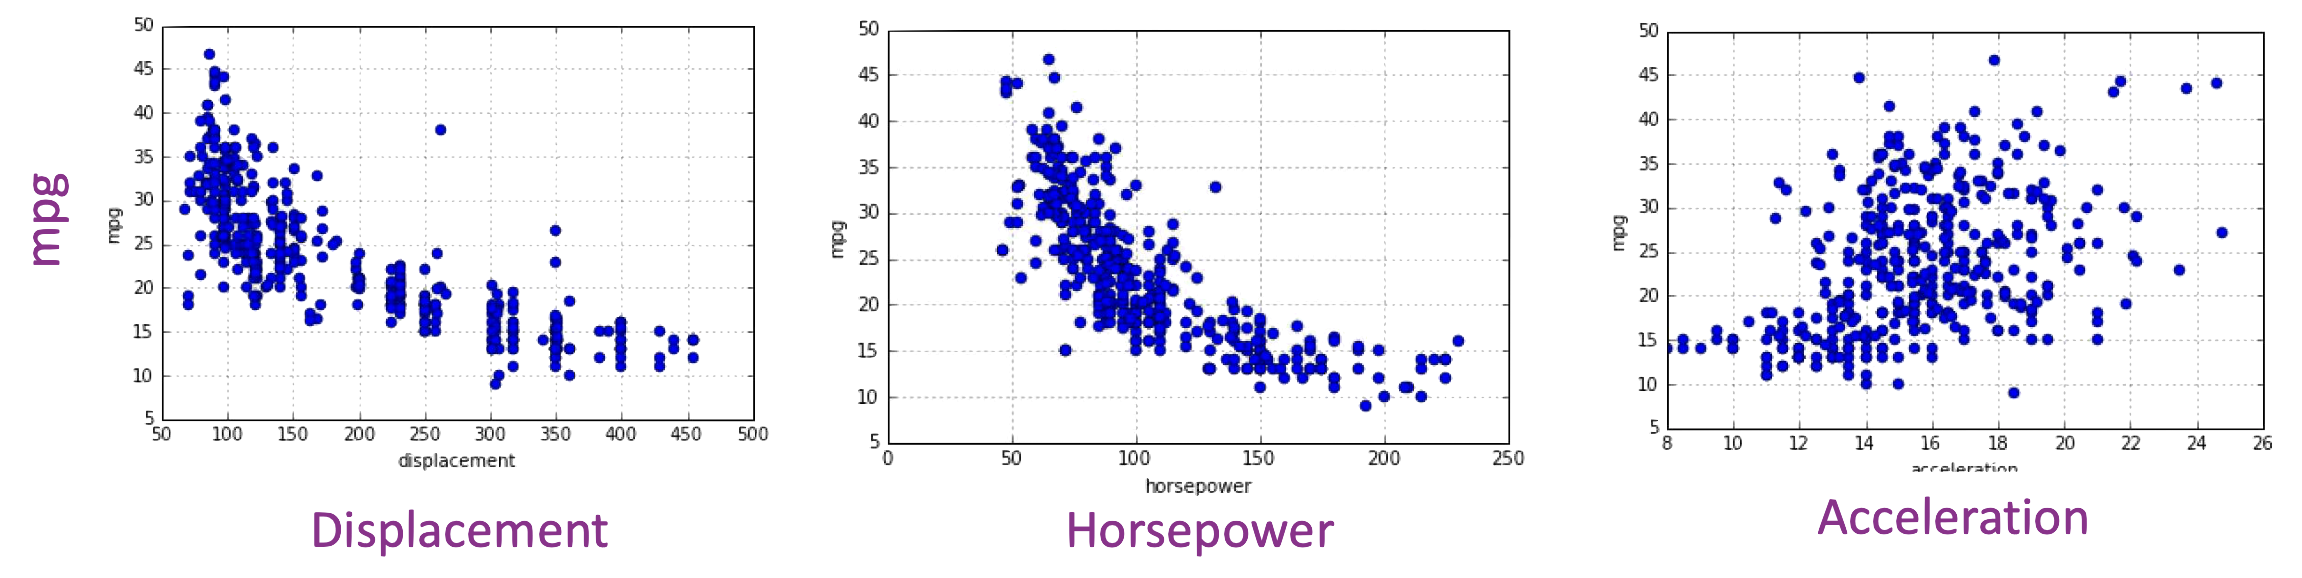
\includegraphics[width=\textwidth]{mpg_plots.png}
	\end{center}
\end{frame}

\begin{frame}
	\frametitle{example from last class}
	\textbf{Dataset:} 
	\vspace{-.5em}
	\begin{itemize}
		\item $x_1, \ldots, x_n \in \R$ (horsepowers of $n$ cars -- this is the predictor/independent variable)
		\item $y_1, \ldots, y_n \in \R$ (MPG -- this is the response/dependent variable)
	\end{itemize}
	\begin{center}
		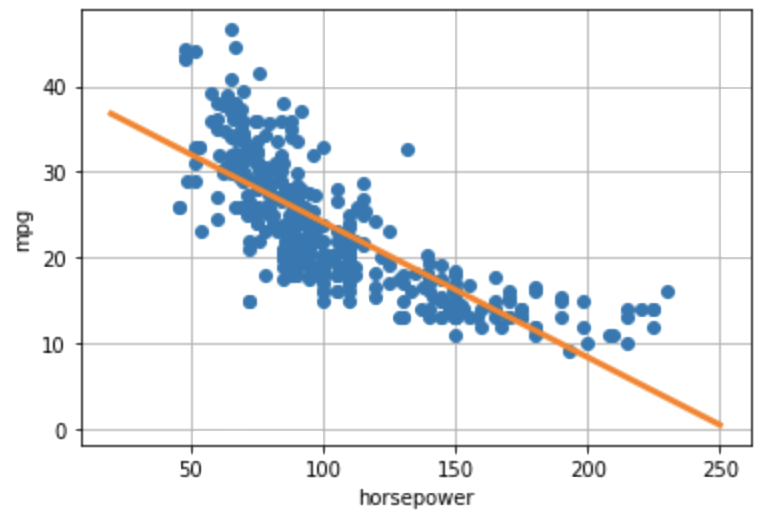
\includegraphics[width=.5\textwidth]{horsepower_fit.png}
	\end{center}
\end{frame}

\begin{frame}
	\frametitle{supervised learning framework}
	\begin{center}
		\textbf{What are the three components needed to setup a supervised learning problem?}
	\end{center}
	\begin{enumerate}
		\item \vspace{1em}
		\item \vspace{3em}
		\item \vspace{3em}
	\end{enumerate}
\end{frame}

\begin{frame}
		\frametitle{supervised learning definitions}
		\small
		\begin{itemize}
			\item \textbf{\alert{Model} $f_{\bs{\theta}}(x)$:} Class of equations or programs which map input $x$ to predicted output. We want $f_{\bs{\theta}}(x_i) \approx y_i$ for training inputs. 
			\item \textbf{\alert{Model Parameters} $\bs{\theta}$:} Vector of numbers. These are numerical nobs which parameterize our class of models.
			\item \textbf{\alert{Loss Function} $L(\bs{\theta})$:} Measure of how well a model fits our data. Typically some function of $f_{\bs{\theta}}(x_1) - y_1, \ldots, f_{\bs{\theta}}(x_n) - y_n$
		\end{itemize}
		\begin{center}
			\textbf{Goal:} Choose parameters $\bs{\theta}^*$ which minimize the Loss Function:
			\begin{align*}
			 	\bs{\theta}^* = \argmin_{\bs{\theta}} L(\bs{\theta})
			\end{align*}
		\end{center}
\end{frame}


\begin{frame}
	\frametitle{linear regression}
			\begin{center}
				\textbf{Linear Regression}
			\end{center}
		
			\begin{itemize}
			\item Model: $f_{\beta_0,\beta_1}(x) = \beta_0 + \beta_1\cdot x$
			\vspace{2em}
			\item Model Parameters: $\beta_0, \beta_1$
			\vspace{2em}
			\item Loss Function: $L(\beta_0,\beta_1) = \sum_{i=1}^n |y_i - f_{\beta_0,\beta_1}(x_i)|^2$ 
			\vspace{2em}
			\end{itemize}

\begin{center}
	\textbf{Goal:} Choose $\beta_0,\beta_1$ to minimize $L(\beta_0,\beta_1) = \sum_{i=1}^n |y_i - \beta_0 - \beta_1x_i|^2$.
\end{center}
\end{frame}

\begin{frame}[t]
	\frametitle{minimizing squared loss for regression}
	 \alert{
	 	\textbf{Claim:} $L(\beta_0, \beta_1)$ is minimized when:
		\begin{itemize}
			\item $\beta_1 = {\sigma_{xy}}/{\sigma_{x}^2}$
			\item $\beta_0 = \bar{y}-\beta_1\bar{x}$
		\end{itemize}
	}
	
	\textbf{Where:} 
	\begin{itemize}
		\item Let $\bar{y} = \frac{1}{n}\sum_{i=1}^n y_i$. \hspace{8.5em}$\bar{y}$ is the \emph{mean} of $y$. 
		\item Let $\bar{x} = \frac{1}{n}\sum_{i=1}^n x_i$. \hspace{8.5em}$\bar{y}$ is the \emph{mean} of $x$. 
		\item Let $\sigma_x^2 = \frac{1}{n}\sum_{i=1}^n (x_i - \bar{x})^2$. \hspace{5em}$\sigma_x^2$ is the \emph{variance} of $x$.
		\item Let $\sigma_{xy} = \frac{1}{n}\sum_{i=1}^n (x_i - \bar{x})(y_i - \bar{y})$. \hspace{2em}$\sigma_{xy} $ is the \emph{covariance}.
	\end{itemize}
\begin{center}
	\textbf{Note:} Only got a nice closed form solution thanks to our choice of loss function. 
\end{center}
	
\end{frame}

\begin{frame}
	\frametitle{a few comments}
	Let $L_{\text{min}} = \min_{\beta_0,\beta_1} L(\beta_0,\beta_1)$.
	\begin{align*}
	R^2 = 1 - \frac{L_{\text{min}}}{n\sigma_y^2} 
	\end{align*}
	is exactly the $R^2$ value you may remember from statistics. A.k.a. the \textbf{``coefficient of determination''}. 
	
	The smaller the loss, the closer $R^2$ is to 1, which means we have a better regression fit. 

\end{frame}

\begin{frame}[t]
	\frametitle{a few comments}
	\textbf{Many reasons you might get a poor regression fit:}
	\begin{center}
		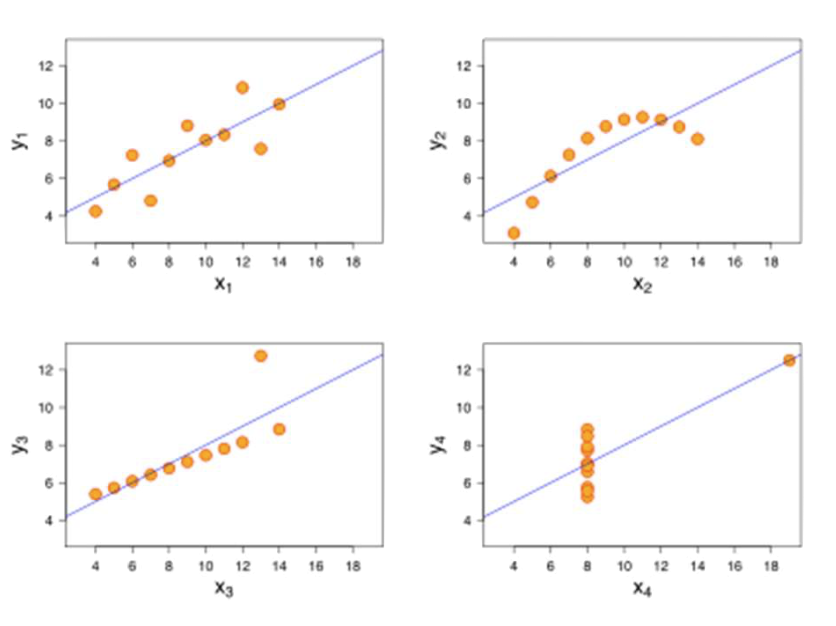
\includegraphics[width=.7\textwidth]{poor_fit.png}
	\end{center}
\end{frame}

\begin{frame}[t]
	\frametitle{a few comments}
	Some of these are fixable!
	\begin{itemize}
		\item Remove outliers, use more robust loss function.
		\item \alert{\textbf{Non-linear model transformation.}}
	\end{itemize}
	Fit the model $\frac{1}{\text{mpg}} \approx \beta_0 + \beta_1\cdot \text{horsepower}$.
	
	\begin{center}
		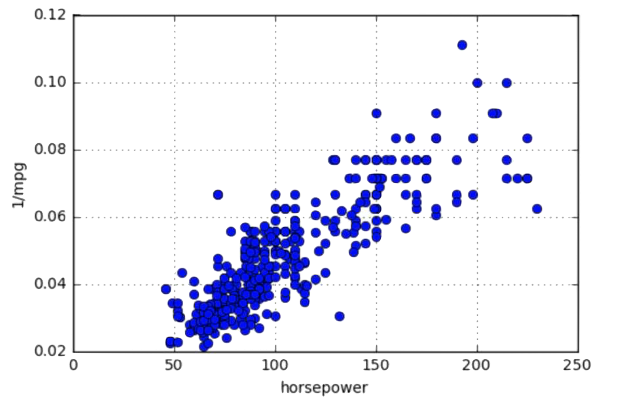
\includegraphics[width=.45\textwidth]{oneovermpg.png}	
	\end{center}
\end{frame}

\begin{frame}[t]
	\frametitle{nonlinear transformation}
	Fit the model $\frac{1}{\text{mpg}} \approx \beta_0 + \beta_1\cdot \text{horsepower}$.

	\begin{itemize}
		\item Set $\tilde{y}_1, \ldots, \tilde{y}_n = 1/y_1, \ldots, 1/y_n$.
		\item Learn function $f$ such that $f(\bv{x}_i)$ predicts $\tilde{y}_i$.
		\item Predict $1/f(\bv{x}_i)$ as MPG for car $i$. 
	\end{itemize}
\end{frame}

\begin{frame}[t]
	\frametitle{nonlinear transformation}
	Fit the model $\frac{1}{\text{mpg}} \approx \beta_0 + \beta_1\cdot \text{horsepower}$.
	
	\begin{itemize}
		\item Set $\tilde{y}_1, \ldots, \tilde{y}_n = 1/y_1, \ldots, 1/y_n$.
		\item Learn function $f$ such that $f(\bv{x}_i)$ predicts $\tilde{y}_i$.
		\item Predict $1/f(\bv{x}_i)$ as MPG for car $i$. 
	\end{itemize}

	\begin{center}
	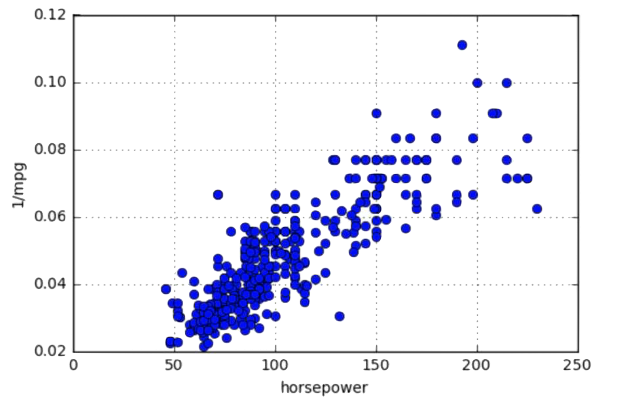
\includegraphics[width=.45\textwidth]{oneovermpg.png}	\includegraphics[width=.45\textwidth]{nonlinear_fit.png}
	
	\textbf{Much better fit, same exact learning algorithm!}
	\end{center}
\end{frame}

\begin{frame}
	\frametitle{multiple linear regression}
	Predict target $y$ using multiple features, simultaneously.
	
	\textbf{Motivating example:} Predict diabetes progression in patients after 1 year based on health metrics. (Measured via numerical score.) \vspace{1em}
	
	\textbf{Features:} Age, sex, body mass index, average blood pressure, six blood serum measurements (e.g. cholesterol, lipid levels, iron, etc.)
	
	\begin{center}
		Demo in \texttt{demo1\_diabetes.ipynb}. 
	\end{center}
\end{frame}

\begin{frame}
	\frametitle{libraries for this demo}
	\begin{center}
		Introducing \textbf{Scikit Learn}.
		
		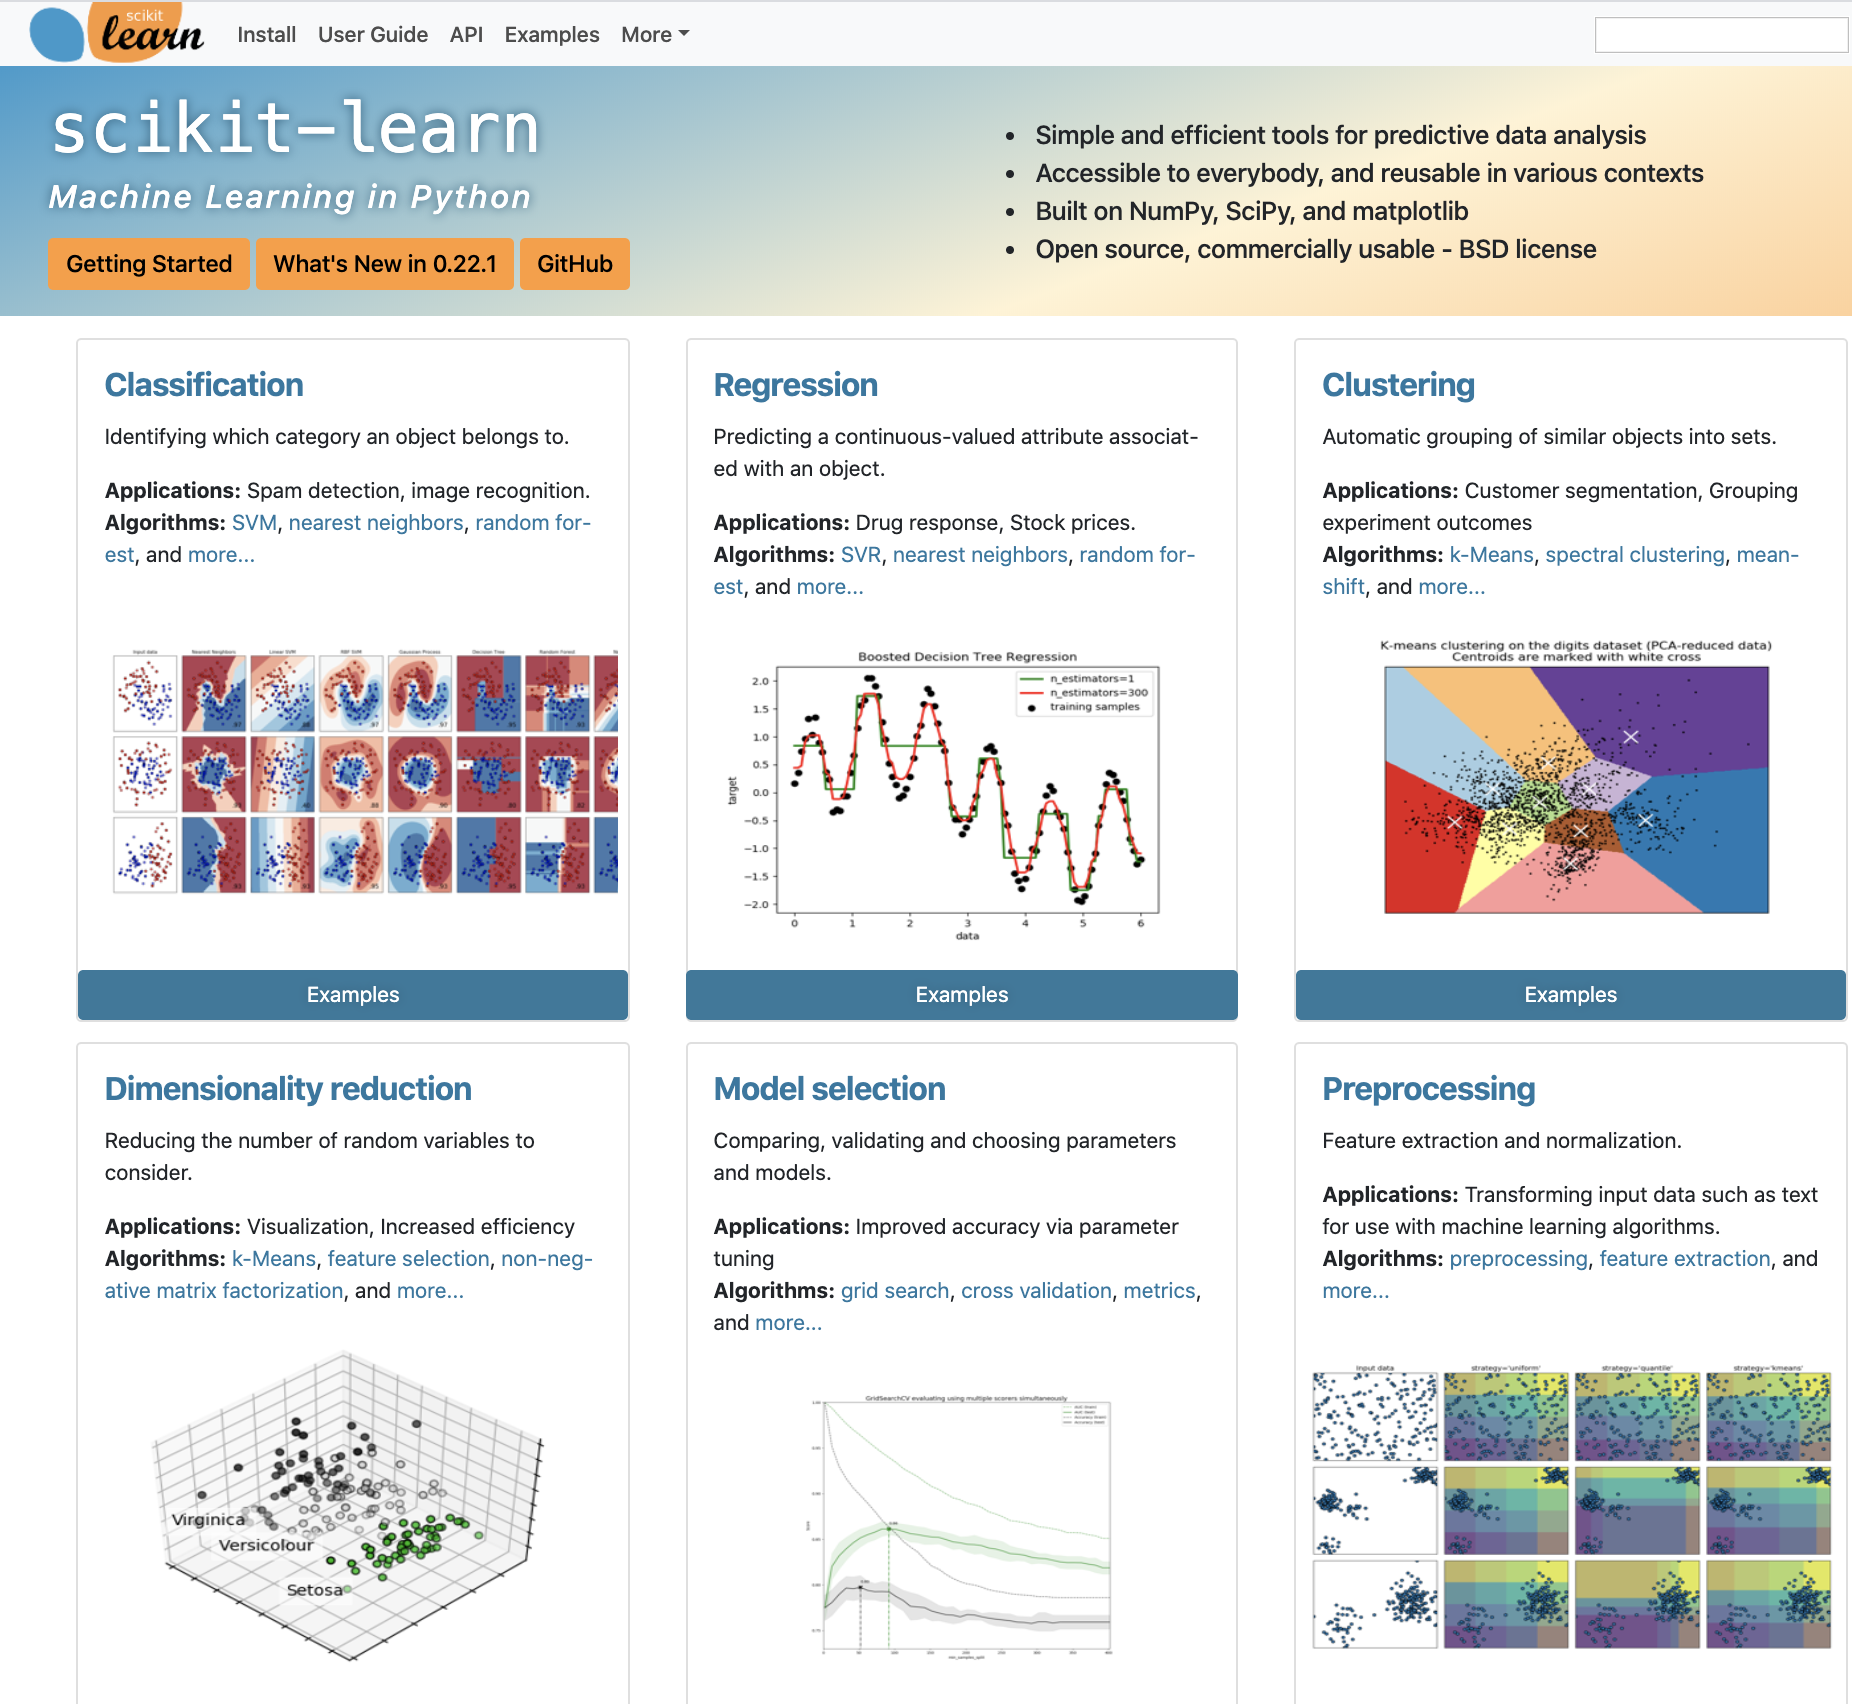
\includegraphics[width=.7\textwidth]{sklearn_web.png}
	\end{center}
\end{frame}

\begin{frame}
	\frametitle{scikit learn}
	\small
	\begin{center}
		
\includegraphics[width=.2\textwidth]{sklearn.png}
	\end{center}
\vspace{-1.5em}
			
	\textbf{Pros:}
	\begin{itemize}
		\item One of the most popular ``traditional'' ML libraries.
		\item Many built in models for regression, classification, dimensionality reduction, etc. 
		\item Easy to use, works with `numpy`, `scipy`, other libraries we use.
		\item Great for rapid prototyping, testing models.
	\end{itemize}
	
	\vspace{-.5em}
	\textbf{Cons:}
	\begin{itemize}
		\item Everything is very ``black-box'': difficult to debug, understand why models aren't working, speed up code, etc.
		\item You will likely want to dive deeper than the built-in functions for your project. 
	\end{itemize}
\end{frame}

\begin{frame}
	\frametitle{scikit learn}
	\textbf{Modules used:}
	\begin{itemize}
		\item \texttt{datasets} module contains a number of pre-loaded datasets. Saves time over downloading and importing with \texttt{pandas}. 
		\item \texttt{linear\_model} can be used to solve Multiple Linear Regression. A bit overkill for this simple model, but gives you an idea of \texttt{sklearn}'s general structure.
	\end{itemize}
\end{frame}

\begin{frame}
	\frametitle{the data matrix}
	\textbf{Target variable:}
	\begin{itemize}
		\item Scalars $y_1, \ldots, y_n$ for $n$ data examples (a.k.a. samples).
	\end{itemize}
	\textbf{Predictor variables:}
	\begin{itemize}
		\item $d$ dimensional vectors $\bv{x}_1, \ldots, \bv{x}_n$ for $n$ data examples and $d$ features
	\end{itemize}
\vspace{-1.5em}

	\begin{center}
		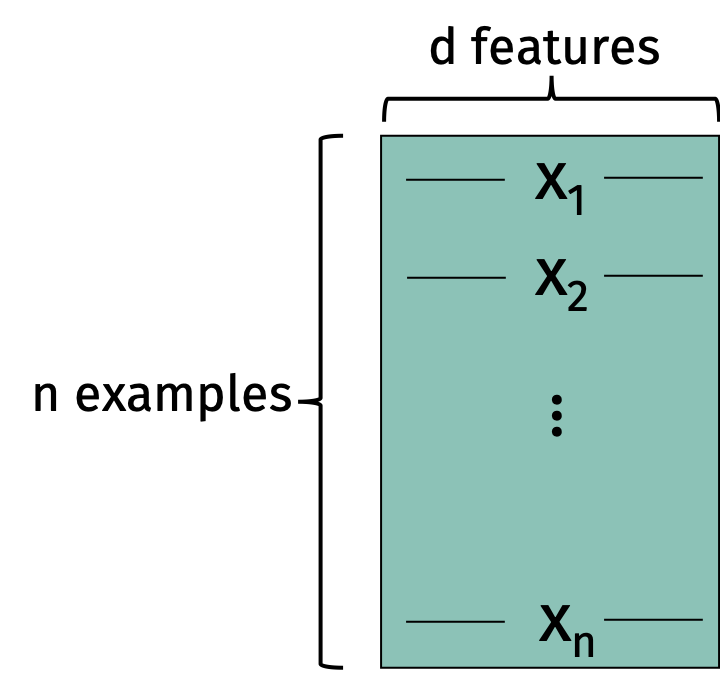
\includegraphics[width=.45\textwidth]{data_matrix_examples.png}
	\end{center}
\end{frame}


\begin{frame}
	\frametitle{the data matrix}
	\textbf{Target variable:}
	\begin{itemize}
		\item Scalars $y_1, \ldots, y_n$ for $n$ data examples (a.k.a. samples).
	\end{itemize}
	\textbf{Predictor variables:}
	\begin{itemize}
		\item $d$ dimensional vectors $\bv{x}_1, \ldots, \bv{x}_n$ for $n$ data examples and $d$ features
	\end{itemize}
\vspace{-1.5em}

	\begin{center}
		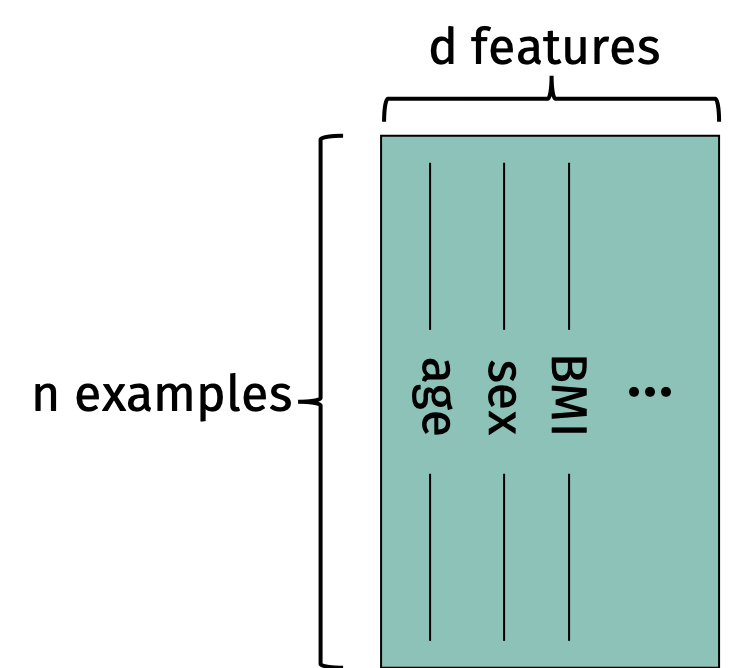
\includegraphics[width=.45\textwidth]{data_matrix_features.png}
	\end{center}
\end{frame}

\begin{frame}
	\frametitle{multiple linear regression}
	\textbf{Data matrix indexing:}
	\begin{align*}
	\bv{X} = \begin{bmatrix}
	\bv{x}_{11} & \bv{x}_{12}  & \ldots &\bv{x}_{1d}\\
	\bv{x}_{21} & \bv{x}_{22}  & \ldots &\bv{x}_{2d}\\
	\bv{x}_{31} & \bv{x}_{32}  & \ldots &\bv{x}_{3d}\\
	\vdots & \vdots  &  &\vdots\\
	\bv{x}_{n1} & \bv{x}_{n2}  & \ldots &\bv{x}_{nd}\\ 
	\end{bmatrix}
	\end{align*}
	\textbf{Multiple Linear Regression Model:}
	\begin{align*}
	&\text{Predict} & y_i &\approx \beta_0 + \beta_1 \bv{x}_{i1} + \beta_2 \bv{x}_{i2} + \ldots + \beta_d \bv{x}_{id}
	\end{align*}
	The rate at which diabetes progress depends on many factors, with each factor having a different magnitude effect.
\end{frame}

\begin{frame}
	\frametitle{multiple linear regression}
	\textbf{Assume first columns contains all $1$'s.} If it doesn't append on a column of all $1$'s.
	\begin{align*}
	\bv{X} = \begin{bmatrix}
	\bv{x}_{11} & \bv{x}_{12}  & \ldots &\bv{x}_{1d}\\
	\bv{x}_{21} & \bv{x}_{22}  & \ldots &\bv{x}_{2d}\\
	\bv{x}_{31} & \bv{x}_{32}  & \ldots &\bv{x}_{3d}\\
	\vdots & \vdots  &  &\vdots\\
	\bv{x}_{n1} & \bv{x}_{n2}  & \ldots &\bv{x}_{nd}\\ 
	\end{bmatrix} = \begin{bmatrix}
	1 & \bv{x}_{12}  & \ldots &\bv{x}_{1d}\\
	1 & \bv{x}_{22}  & \ldots &\bv{x}_{2d}\\
	1 & \bv{x}_{32}  & \ldots &\bv{x}_{3d}\\
	\vdots & \vdots  &  &\vdots\\
	1 & \bv{x}_{n2}  & \ldots &\bv{x}_{nd}\\ 
	\end{bmatrix}
	\end{align*}
	\vspace{1em}
	\textbf{Multiple Linear Regression Model:}
	\begin{align*}
	&\text{Predict} & y_i &\approx \beta_1 \bv{x}_{i1} + \beta_2 \bv{x}_{i2} + \ldots + \beta_d \bv{x}_{id}
	\end{align*}
\end{frame}


\begin{frame}
	\frametitle{multiple linear regression}
			\begin{center}
				\textbf{Use as much linear algebra notation as possible!}
			\end{center}

			\begin{itemize}
				\item Model: 
				\vspace{4em}
				\item Model Parameters: 
				\vspace{4em}
				\item Loss Function:
				\vspace{4em}
			\end{itemize}
\end{frame}

\begin{frame}
	\frametitle{multiple linear regression}
	\begin{center}
		\textbf{Linear \emph{Least-Squares} Regression.}
	\end{center}
	\begin{itemize}
		\item Model: 
		\begin{align*}
		f_{\bs{\beta}}(\bv{x}) = \langle\bv{x},\bs{\beta}\rangle
		\end{align*}
		\item Model Parameters: 
		\begin{align*}
		\bs{\beta} = \left[\beta_1, \beta_2, \ldots, \beta_d \right]
		\end{align*}
		\item Loss Function:
		\begin{align*}
		L(\bs{\beta}) = &\sum_{i=1}^n |y_i - \langle\bv{x}_i,\bs{\beta}\rangle|^2 \\
		& = \|\bv{y} -\bv{X}\bv{\beta}\|_2^2
		\end{align*}
	\end{itemize}
\end{frame}

\begin{frame}
	\frametitle{linear algebraic form of loss function}
	
	
\end{frame}

\begin{frame}
	\frametitle{loss minimization}
	\textbf{Machine learning goal:} minimize the loss function $L(\bs{\beta}): \R^{d} \rightarrow \R$.
	
	\vspace{1em}
	Find optimum by determining for which $\bs{\beta} = [\beta_1, \ldots, \beta_d]$ all partial derivatives are $0$. I.e. when do we have:
		\begin{align*}
		\begin{bmatrix}
		\frac{\partial L}{\partial \beta_1} \\ \frac{\partial L}{\partial \beta_2} \\ \vdots \\ \frac{\partial L}{\partial \beta_d}
		\end{bmatrix} = 
		\begin{bmatrix}
		0 \\ 0 \\ \ldots \\ 0
		\end{bmatrix} 
		\end{align*}
\end{frame}

\begin{frame}
	\frametitle{gradient}
	For any function $L(\bs{\beta}): \R^{d} \rightarrow \R$, $\nabla L(\beta)$ is a function from $\R^d \rightarrow \R^d$ defined:
	\begin{align*}
	\nabla L(\beta) = \begin{bmatrix}
	\frac{\partial L}{\partial \beta_1} \\ \frac{\partial L}{\partial \beta_2} \\ \vdots \\ \frac{\partial L}{\partial \beta_d}
	\end{bmatrix}
	\end{align*}
	The \emph{gradient} of the loss function is a central tool in machine learning. We will use it again and again. 
\end{frame}

\begin{frame}[t]
	\frametitle{gradient}
	\textbf{Loss function:}
	\begin{align*}
	\|\bv{y} - \bv{X}\bs{\beta}\|_2^2
	\end{align*}
	
	\textbf{Gradient:}
	\begin{align*}
	-2\cdot \bv{X}^T(\bv{y} - \bv{X}\bs{\beta})
	\end{align*}
	
\end{frame}

\begin{frame}[t]
	\frametitle{gradient warmup}
	
\end{frame}



\begin{frame}[t]
	\frametitle{gradient derivation}
	\begin{center}
	\textbf{Loss function:} $\|\bv{y} - \bv{X}\bs{\beta}\|_2^2$. 
	\end{center}
	
\end{frame}

\begin{frame}[t]
		\frametitle{loss minimization}
	\textbf{Goal:} minimize the loss function $L(\bs{\beta}) = \|\bv{y} - \bv{X}\bs{\beta}\|_2^2$.
	
	\begin{align*}
	-2\cdot \bv{X}^T(\bv{y} - \bv{X}\bs{\beta}) = \bv{0}
	\end{align*}
	
	\textbf{Solve for optimal $\bs{\beta}^*$:}
	\begin{align*}
	\bv{X}^T\bv{X}\bs{\beta}^* &= \bv{X}^T\bv{y} \\
	\alert{\bs{\beta}^*} &\alert{= \left(\bv{X}^T\bv{X}\right)^{-1}\bv{X}^T\bv{y}}
	\end{align*}
\end{frame}

\begin{frame}[t]
	\frametitle{multiple linear regression solution}
	Need to compute $\bs{\beta}^* = \argmin_{\bs{\beta}}\|\bv{y} - \bv{X}\bs{\beta}\|_2^2 = \left(\bv{X}^T\bv{X}\right)^{-1}\bv{X}^T\bv{y}$.
	\begin{itemize}
		\item Main cost is computing $(\bv{X}^T\bv{X})^{-1}$ which takes $O(nd^2)$ time. 
		\item Can solve slightly faster using the method \texttt{numpy.linalg.lstsq}, which is running an algorithm based on QR decomposition. 
		\item For larger problems, can solve \emph{much faster} using an \textit{iterative methods} like \texttt{scipy.sparse.linalg.lsqr}.
	\end{itemize}

\begin{center}
	Will learn more about iterative methods when we study \emph{Gradient Descent}.
\end{center}
\end{frame}

\begin{frame}
	\frametitle{test your intuition}
	What is the sign of $\beta_1$ when we run a \emph{simple} linear regression using the following predictors in isolation:
	\begin{itemize}
		\item Body mass index (BMI): \textbf{positive}
		\item Sex (values of 1 indicates male, value of 2 indicates female): \textbf{positive}
	\end{itemize}

	What is the sign of the corresponding $\beta$'s when we run a \emph{multiple} linear regression using the following predictors together:
	\begin{itemize}
	\item Body mass index (BMI): \textbf{positive}
	\item Sex (values of 1 indicates male, value of 2 indicates female): \textbf{negative}
	\end{itemize}
	\begin{center}
		\alert{\textbf{Can you explain this? What are other examples when this phenomenon might show up?}}
	\end{center}
\end{frame}

\begin{frame}
	\frametitle{transformed linear models}
	How could we fit the \emph{non-linear} model:
	\begin{align*}
	y_i \approx \beta_0 + \beta_1 x_i +  \beta_2 x_i^2 +  \beta_3 x_i^3.
	\end{align*}
	\begin{center}
		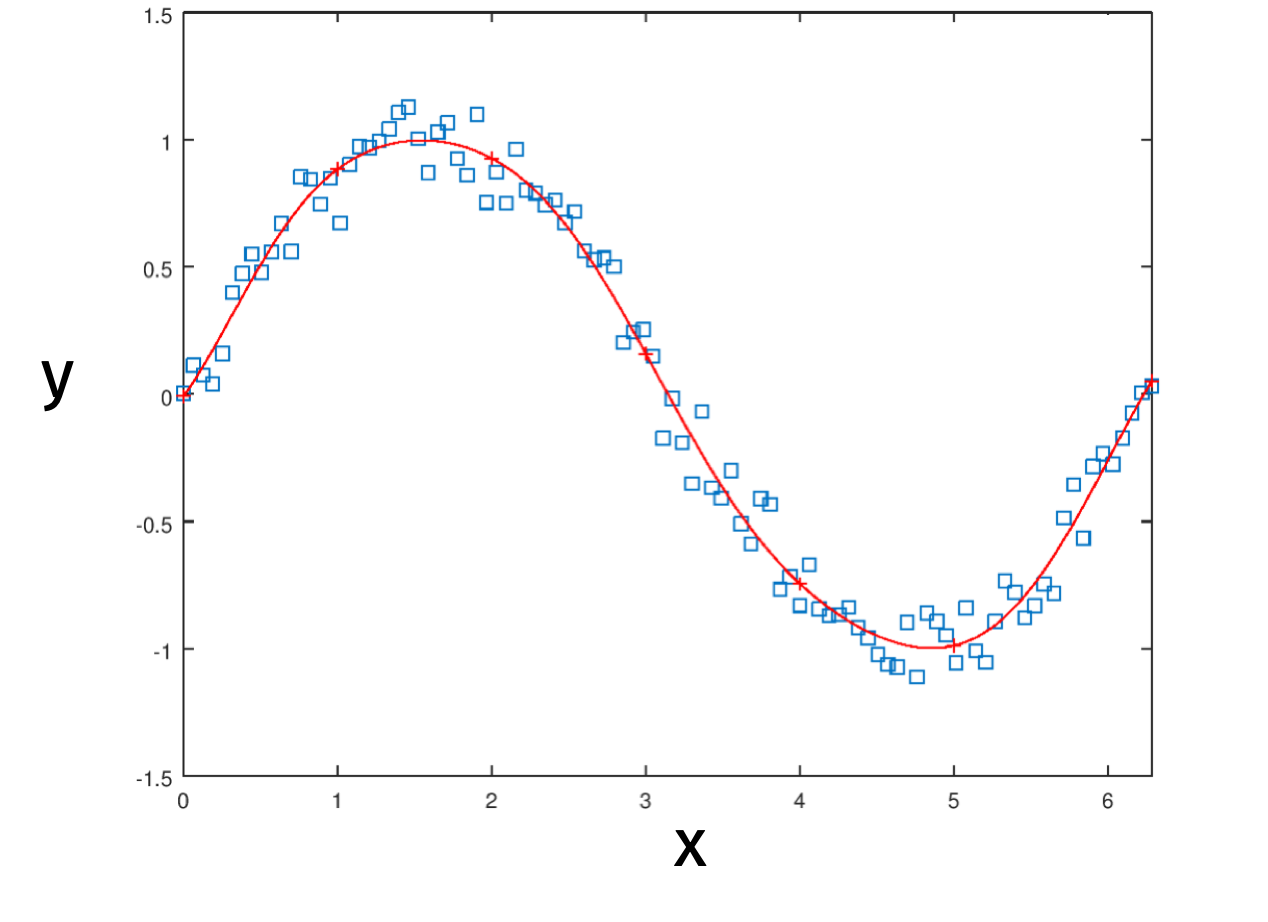
\includegraphics[width=.6\textwidth]{poly_fit.png}
	\end{center}
\end{frame}

\begin{frame}
	\frametitle{transformed linear models}
	Transform into a multiple linear regression problem:
	\begin{align*}
	\textbf{X} = \begin{bmatrix}
	1 & x_1  &  x_1^2 & x_1^3\\
	1 & x_2  &  x_2^1 &  x_2^3 \\
	1 & x_3  &  x_3^2 &  x_3^3\\
	\vdots & \vdots  &  &\vdots\\
	1 & x_n  &  x_n^2 & x_n^3\\ 
	\end{bmatrix}
	\end{align*}
	Each column $j$ is generated by a different basis function $\phi_j(x)$. Could have:
	\begin{itemize}
		\item $\phi_j(x) = x^q$
		\item $\phi_j(x) = sin(x)$
		\item $\phi_j(x) = cos(10)$
		\item $\phi_j(x) = 1/x$
	\end{itemize}
\end{frame}

\begin{frame}
	\frametitle{transformed linear models}
	Suppose we go back to the MPG prediction problem. What if we had a \emph{categorical} random variable for car make: e.g. Ford, BMW, Honda. \textbf{How would you encode as a numerical column?}
		\begin{align*}
		\begin{bmatrix}
		\texttt{ford} \\\texttt{ford} \\ \texttt{honda} \\ \texttt{bmw} \\ \texttt{honda} \\ \texttt{ford}
		\end{bmatrix} \rightarrow 
		\begin{bmatrix}
		\hspace{2em} \\\hspace{2em} \\ \hspace{2em} \\ \hspace{2em} \\ \hspace{2em} \\ \hspace{2em}
		\end{bmatrix}
		\end{align*}
\end{frame}

\begin{frame}
	\frametitle{one hot encoding}
	\textbf{Better approach:} \emph{One Hot Encoding.}
			\begin{align*}
	\begin{bmatrix}
	\texttt{ford} \\\texttt{ford} \\ \texttt{honda} \\ \texttt{bmw} \\ \texttt{honda} \\ \texttt{ford}
	\end{bmatrix} \rightarrow 
	\begin{bmatrix}
	1 & 0 & 0 \\1 & 0 & 0 \\ 0 & 1 & 0 \\ 0 & 0 & 1\\ 0 & 1 & 0 \\ 1 & 0 & 0
	\end{bmatrix}
	\end{align*}
	\begin{center}
		\alert{\textbf{Avoids adding inadvertent linear relationships.}}
	\end{center}
\end{frame}

\end{document} 








